%!xelatex = 'xelatex --halt-on-error %O %S'
\documentclass{thuemp}
\begin{document}
\emptitle{OS代码阅读报告}
\empauthor{江灿}{2019011325}
\fancyhead[CO]{{\footnotesize 江灿: Os代码阅读报告}}
\Keyword{光栅衍射,波长,光栅常数,最小偏向角}
\twocolumn[
\begin{@twocolumnfalse}
\maketitle
\begin{empAbstract}
	本次实验是
\end{empAbstract}
% \empfirstfoot{2022-04-03}{软件02}{双日下M}{7号}
\end{@twocolumnfalse}
]
%%%%%%%%%%%%%%%%%%%%%%%%%%%%%%%%%%%%%%%%%%%%%%%%%%%%%%%%%%%%%%%%
%%%%%%%%%%%%%%%%%%%%%%%%%%%%%%%%%%%%%%%%%%%%%%%%%%%%%%%%%%%%%%%%
%%%%%%%%%%%%%%%%%%%%%%%%%%%%%%%%%%%%%%%%%%%%%%%%%%%%%%%%%%%%%%%%
%  正文由此开始
\wuhao 
代码报告基本要求
\begin{itemize}
  \item 重要函数或语句的代码分析与注释
  \item 基本流程分析
  \item 实现概述
  \item 阅后心得
  \item 评分:知识的理解程度,主要技术分析程度,认真程度
\end{itemize}
\part*{Chapter 1 Operatings system interfaces}
\section*{preface}
The job of an operating system is to share a computer among multiple programs and to provide a more useful set of services than the hardware alone supports.And provides services to user programs through an interface\\
\subsection*{What is a good interface :} provides services to user programs through an interface;offer many powerful features to applications\\
\textbf{xv6:}mimicking Unix's internal design\\
knrnel:a special program that provides services to running programs\\
program(called a process):has memory containing instructions, data, and a stack\\
instructions:implement the program’s computation\\
data:variables on which the computation acts\\
stack:organizes the program’s procedure calls
\begin{figure}[H]
	\centering
	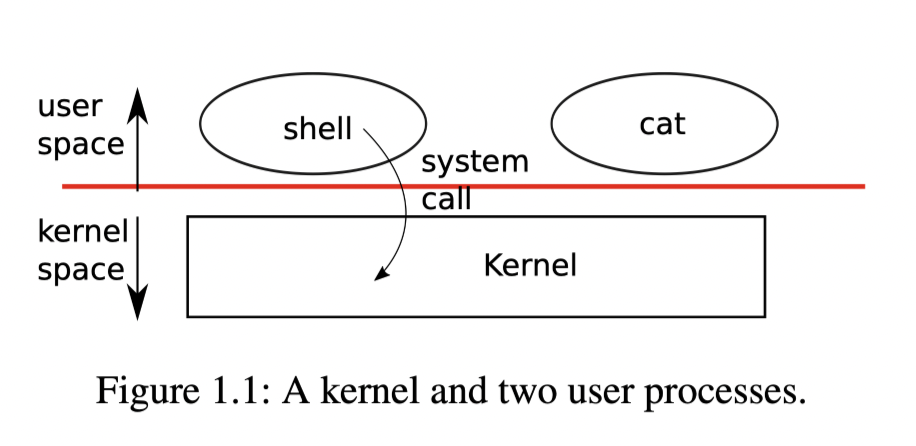
\includegraphics[width=0.8\linewidth]{./image/1.1.png}
	\caption{A kernel and two user processes} 
	\label{png:1.1}
\end{figure}
shell:an ordinary program that reads commands 
from the user and executes them.
The fact that the shell is a user program, 
and not part of the kernel

%  分栏开始
















\newpage
% \begin{figure}[H]
% 	\centering
% 	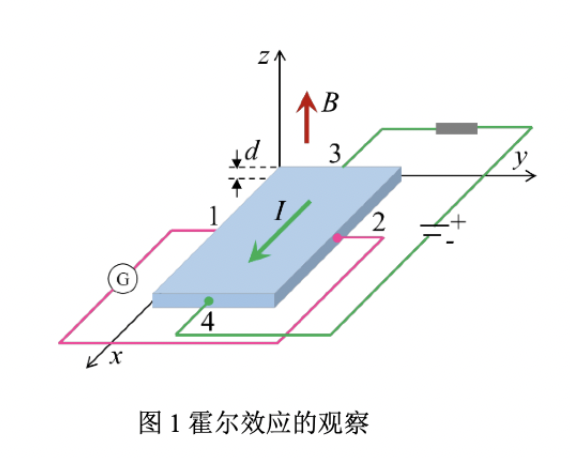
\includegraphics[width=0.8\linewidth]{./image/1.png}
% 	\caption{测定光栅常数和光波波长数据} 
% 	\label{png:1}
% \end{figure}








%%%%%%%%%%%%%%%%%%%%%%%%%%%%%%%%%%%%%%%%%%%%%%%%%%
%  参考文献
%%%%%%%%%%%%%%%%%%%%%%%%%%%%%%%%%%%%%%%%%%%%%%%%%%%%%%%%%%%%%%%%
%  参考文献按GB/T 7714-2015《文后参考文献著录规则》的要求著录. 
%  参考文献在正文中的引用方法:\cite{bib文件条目的第一行}

\renewcommand\refname{\heiti\wuhao\centerline{参考文献}\global\def\refname{参考文献}}
\vskip 12pt

\let\OLDthebibliography\thebibliography
\renewcommand\thebibliography[1]{
  \OLDthebibliography{#1}
  \setlength{\parskip}{0pt}
  \setlength{\itemsep}{0pt plus 0.3ex}
}

{
\renewcommand{\baselinestretch}{0.9}
\liuhao
\bibliographystyle{gbt7714-numerical}
\bibliography{./TempExample}
}


\end{document}
